%! TeX root = thesis.tex
\chapter{Background}
\tikzset{HighLevelProcedure/.pic={
	\def\dx{6mm}
	% nodes
	\node[] (Mesh) {Mesh};
	\node[FC-Node] (3DSeg) [right=\dx of Mesh] {3D Segmentation};
	\node[FC-Node] (GeoSimp) [right=\dx of 3DSeg] {Geometry Simplification};
	\node[FC-Node] (2DSeg) [right=\dx of GeoSimp] {2D Segmentation};
	\node[FC-Node,text width=27mm] (Bpath) [below=10mm of Mesh, xshift=10mm] {Cellular path planning};
	\node[FC-Node,text width=30mm] (TSP) [right=\dx of Bpath] {Modified TSP};
	\node[FC-Node,text width=20mm] (InvKin) [right=\dx of TSP] {Inverse Kinematics};
	\node[text width=20mm] (Poses) [right=\dx of InvKin] {Actuator Poses};
	% connections
	\draw [FC-Arrow] (Mesh) -- (3DSeg);
	\draw [FC-Arrow] (3DSeg) -- (GeoSimp);
	\draw [FC-Arrow] (GeoSimp) -- (2DSeg);
	\draw [FC-Arrow, rounded corners=5pt] (2DSeg.south) |-| (Bpath.north);
	\draw [FC-Arrow] (Bpath) -- (TSP);
	\draw [FC-Arrow] (TSP) -- (InvKin);
	\draw [FC-Arrow] (InvKin) -- (Poses);
}}

\begin{figure}[hb]
	\centering
\begin{tikzpicture}
	\pic at (0,0) {HighLevelProcedure};
\end{tikzpicture}
	\caption{Graphical overview of the path planning and execution procedure}
	\label{fig:bkgd_overview}
\end{figure}
The objective is to plan a path covering the surface of an unknown object.
The intended application of this is to be able to clean a surface via ablation using a planar laser.
The general flow (? procedure?) presented in this work is as follows.
The high level procedure is shown in Figure \ref{fig:bkgd_overview}
The 3D triangular mesh of an object is provided as input.
This mesh is segmented using Watershed segmentation into regions of low curvature separated by regions of high curvature.
These regions are classified into different categories of geometric primitives, or if no classification is possible, subjected to Watershed segmentation again.
Once all regions have been classified, idealized geometric representations, termed ``simple surfaces'', are created from each based on their primitive classification.
Non-convex simple surfaces are subject to 2D segmentation, from which convex sub-regions are produced.
A local coverage path is then planned on each convex region.
The task of combining the individual paths into a single path is a form of Traveling Salesman Problem (TSP).
Once the path is complete, the waypoints thereof may be sent to the robot arm tasked with carrying out the cleaning operation.

\section{A Note on Notation}
To transforma a point from one coordinate system to another one typically uses a transformation matrix, denoted $T$.
There is no unified notation to indicate in which coordinate system a point resides, nor is there to indicate from which to which coordinate systems a $T$ will transform.
% There is no unified notation for $T$ to indicate its source and target coordinate systems.
In order to dispell any confusion, the notation used in this work is explained below.
As is typical, right subscripts are used to indicate information about the owning quantity.
To indicate the coordinate system in which point or vector exists, the left superscript is used.
\begin{equation*}
	\prescript{0}{}p_i
\end{equation*}
represents the $i$-th point in coordinate system 0 (shorthand for global coordinate system).
For transformation matrices the right subscript is designates the \textit{source} coordinate system, and the left superscript the \textit{target} coordinate system.
This leaves the right superscript position open for a transpose or inverse symbol.
\begin{equation*}
	\prescript{0}{}T_{A}
\end{equation*}
gives a transformation matrix from the \textit{A} coordinate system to the global coordinate system.
This schema provides an inherent check that multiplication between two quantities is valid according to their frames of reference.
\begin{equation*}
	\prescript{0}{}p_i = \prescript{0}{}T_{A} \prescript{A}{}p_i
\end{equation*}
shows the transformation of point $p_i$ in coordinate system $A$ to the global coordinate system.
In this last example the coordinate system of $p_i$ and the source coordinate system of $T$ appear adjacent and near vertical of one another, confirming that this is a valid transformation.

\section{Geometric Curvature}
The first step of \textit{3D Segmentation} is to segment the object's mesh using Watershed segmentation.
Watershed segmentation requires a ``height'' function be applied to each vertex of the given mesh.
See Section \ref{sec:ws_seg} for greater detail on Watershed segmentation.
In order to segment the mesh along regions of high curvature, the vertice's height must be a function of its curvature.
The various forms and types of curvature examined throughout this project are presented in the following sections.

Curvature descibes the rate of change of a curve or surface's tangent.
Figure \ref{sfig:tangent_on_curve} shows the curvature $\kappa$ as the change of the tangent at the marked point as it moves along the curve.
Alternatively, the curvature of a point on a surface can be defined via the osculating circle at that point, which is the circle that best approximates the surface at that point.
Following that definition, the curvature is the inverse radius of the osculating circle.

\begin{figure}[ht]
	\centering
	\begin{subfigure}{0.47\textwidth}
		\centering
\begin{tikzpicture}[scale=1.5]
	% based on image in slide 22/23 in DDG-Curves.pdf
	% \draw[step=10mm,gray!50,very thin] (-0.2,-0.2) grid (5.2,3.2);
	\draw[] (-0.1,-0.1) .. controls (2.0,2.0) and (2.5,0) .. (1.5,0)
		% node [sloped,pos=0.1,minimum size=10mm,anchor=south west] (pt1) {}
		% node [sloped,pos=0.15,minimum size=9mm,anchor=south west] (pt1d) {}
		node [sloped,pos=0.38,minimum size=15mm,anchor=south west] (pt2) {}
		node [sloped,pos=0.43,minimum size=12mm,anchor=south west] (pt2d) {};
	% Point 1
	% \fill (pt1.south west) circle[radius=2pt,blue];
	% \path (pt1.south west) edge[-Stealth] node[above] {$\vec{t}$} (pt1.south east);
	% Point 1 delta and curvature
	% \path (pt1d.south west) edge[-Stealth] node[] {} (pt1d.south east);
	% \draw[dashed] (pt1.south east) -- (pt1d.south east) node[pos=0.5] {$\kappa$};
	% Point 2
	\fill (pt2.south west) circle[radius=1.5pt,blue];
	\path (pt2.south west) edge[-Stealth] node[above] {$\vec{t}$} (pt2.south east);
	% Point 2 delta and curvature
	\path (pt2d.south west) edge[-Stealth] node[] {} (pt2d.south east);
	\draw[red] (pt2.south east) -- (pt2d.south east) node[pos=0.5,anchor=west] {$\kappa$};
\end{tikzpicture}
		\caption{%
Normal vector of a point on a curve.
Inspired by~\cite{DDGAppIntro_12_smooth_curves}.}
		\label{sfig:tangent_on_curve}
	\end{subfigure}
	\hfill
	\begin{subfigure}{0.45\textwidth}
		\centering
	\includegraphics[width=0.7\textwidth]{../resources/curvature/osculating_circle.png}
% \begin{tikzpicture}[scale=1.0]\end{tikzpicture}
		\caption{%
A curve with osculating circle at point $p$.
Image from~\cite{DDGAppIntro_12_smooth_curves}, unless replaced by TikZ.
(? TODO: recreate important parts in TikZ)
}
		% \label{sfig:mesh_neighborhood}
	\end{subfigure}
	% \caption{}
\end{figure}

\subsection{Principal Curvatures}
All combined measures of curvature are based, either in theory or in actuality, on the principal curvatures.
The principal curvatures at a given point on a surface are simply the maximum $\kappa_1$ and minimum $\kappa_2$ curvature~\cite{DDGAppIntro_17_smooth_k}.
Note that in this work the first principal curvature is the maximum and the second the minimum, whereas other sources may use the reverse schema.
The principal curvatures at the top of a hill-like surface are illustrated in Figure \ref{fig:principal_k}.

\begin{figure}[htb]
	\centering
	% \includegraphics[width=0.7\textwidth]{../resources/minimal_surface_curvature_planes-en.svg.png}
	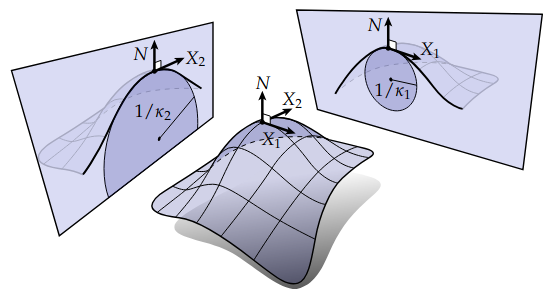
\includegraphics[width=0.7\textwidth]{../resources/curvature/principal_curvatures.png}
	% \includesvg[width=0.9\textwidth]{../resources/Minimal_surface_curvature_planes-en.svg}
	\caption{
Principal curvatures are shown on an ellipsoidally round surface~\cite{Digital_geom_proc_w_disc_ext_calc}.
$X_1$ and $X_2$ show the principal directions.
The cutaway views show this as an osculating circle in each projection of the surface.
}
	\label{fig:principal_k}
\end{figure}

Determining principal curvatures for a continuous surface is unambiguous.
The principal curvatures of a surface $S$ at point $p$ are defined by the 2nd fundamental form~\cite{DiffGeo_curves_surfaces, Basic_diff_geo_of_surfaces, DDGAppIntro_17_smooth_k} $\textbf{II}(X,Y)$, where $X$ and $Y$ are orthonormal vectors at $p$.
\iffalse
\begin{equation}
	\textbf{II}(U,V) = Ldu^2 + 2 M du dv + N dv^2,%\langle dN(X), df(Y)\rangle,
\end{equation}
where $U$ and $V$ are orthonormal vectors tangent to the point $(u,v)$ on some surface, $du$ and $dv$ are the changes in the $U$ and $V$ directions, repsectively.
Additionally, $L$ is ...
and can be found as the eigenvalues of
\fi
The principal curvatures are the eigenvalues of
\begin{equation}\label{eq:2nd_fundamental_tensor}
	\begin{bmatrix}
		\textbf{II}(X_1, X_2) & \textbf{II}(X_1, X_2) \\
		\textbf{II}(X_2, X_1) & \textbf{II}(X_2, X_2)
	\end{bmatrix},
\end{equation}
where $X_1$ and $X_2$ are the aforementioned orthonormal vectors tangent to the surface at point $p$.
Similarly, the principal directions are the eigenvectors of Equation \ref{eq:2nd_fundamental_tensor}.

There are however various ways of approximating the principal curvatures on a discrete mesh~\cite{EstCurvOnTriMesh, DiscDiffGeoOpsTriMani}.
A basic approach is to calculate the mean and Gaussian curvatures, and derive the principal curvatures from them~\cite{DDGAppIntro_19_discrete_k_2, Gauss_mean_k_notes}.
Given the mean curvature $H$ and Gaussian curvature $K$ (see Sections \ref{sec:mean_k} and \ref{sec:gauss_k}), the principal curvatures can be calculated from Equations \ref{eq:mean_k} and \ref{eq:gauss_k}, or the discrete approximations from Equations \ref{eq:dihedral_angle} and \ref{eq:disc_gauss_k}.
\begin{align*}
	\kappa_1 &= H - \sqrt{H^2 - K} \\
	\kappa_2 &= H + \sqrt{H^2 - K}
\end{align*}
Although theoretically impossible, discretization errors can cause $H^2$ to be less than $K$, resulting in ``imaginary'' curvature.
This tends to occur on planar mesh regions, thus a minimum of 0 can be set for $H^2 - K$, because the root term would have been near 0 regardless, but it does highlight a flaw in this measure of curvature.

Initially, RMS curvature calculated from discrete Gaussian and mean curvature was used as the mesh height.
But this was eventually replaced with Taubin's method of calculating the principal curvatures directly via curvature tensor estimation~\cite{TaubinTensor}.
This has the benefit of direct calculation, but has been shown to be succeptible to noise in the mesh~\cite{Comp_k_notes}.
% Thiesel et al. calculate the curvature tensor per triangular face in the mesh, based on the face's corner normals~\cite{Norm_based_k_tensor_est}.
This too was later retired, and replaced with Rusinkiewicz's approach of calculating the curvature tensor for each mesh face via the differences between corner normals~\cite{SRTensor}, then computing the per vertex curvature tensor as a weighted sum over the curvature tensors of the vertex's adjoining triangles via coordinate system transformations.
% Gatzke and Grimm examine a variety of other curvature estimation methods~\cite{EstCurvOnTriMesh}, most of which were not considered for this work.

\subsection{Mean Curvature}\label{sec:mean_k}
The discrete mean curvature was used early in development as part of the RMS curvature calculation.
Mean curvature is, as the name implies, the mean of the principal curvatures~\cite{DDGAppIntro_19_discrete_k_2}
\begin{equation}\label{eq:mean_k}
	H = \frac{\kappa_1 + \kappa_2}{2}
\end{equation}
where $H$ is the mean curvature.
Mean curvature can be approximated on a discrete mesh via sum of dihedral edge angle length products:
\begin{equation}\label{eq:dihedral_angle}
	H_i := \frac{1}{2}\sum_{j \in E}l_{ij} \phi_{ij}
\end{equation}
where $H_i$ is the mean curvature at vertex $i$, $j$ is a vertex in the ring of $i$, $l_{ij}$ is the length of the edge from $i$ to $j$, and $\phi_{ij}$ is the dihedral angle between the faces adjacent to edge $ij$.
See Figure \ref{sfig:dihedral_angle} for a graphic depiction.

Alternatively, the mean curvature normal $\Delta f$ can be calculated via the discrete Laplace-Beltrami operator~\cite{DDGAppIntro_18_discrete_k_1}
\begin{equation}\label{eq:lap_beltrami_op}
	(\Delta f)_i := \frac{1}{2}\sum_{j \in E}(\cot \alpha_{ij} + \cot \beta_{ij})(p_j - p_i),
\end{equation}
and the absolute mean curvature can be calculated as half of the magnitude thereof
\begin{equation}
	|H_i| = \frac{\|(\Delta f)_i \|}{2}.
\end{equation}
In Equation \ref{eq:lap_beltrami_op} above $p_j$ is a vertex in the ring of vertex $p_i$ which indicates the current edge, $\alpha_{ij}$ and $\beta_{ij}$ are the angles opposite the current edge (see \ref{sfig:mesh_neighborhood}).

\begin{figure}[htb]
	\centering
	\begin{subfigure}[t]{0.47\textwidth}
		\centering
\begin{tikzpicture}[
	hidden/.style={inner sep=0, outer sep=0}]
	\node [vertex,label=180:i] (node_i) at (-0.4,2.2) {};
	\node [vertex,label=215:j] (node_j) at (0.4,-2.2) {};
	\node [hidden] (node_l) at (-2.3,-0.8) {};
	\node [hidden] (node_r) at (1.7,0.5) {};
	\draw (node_i) -- (node_j) -- (node_r) -- (node_i) -- (node_l) -- (node_j);
	\draw [dashed,gray!60] (node_l) -- (node_r);
	% try to draw curved arrow
	\draw [-Stealth,thick] (20:4mm) arc [start angle=20, delta angle=-180, x radius=5mm, y radius=3mm];
		% node [pos=0.8, label={250:$\phi_{ij}$}] {};
	\node [] at (-0.3, -0.6) {$\phi_{ij}$};
	\draw [|-|, thick] ($(node_i.east)+(0.1,0.05)$) -- ($(node_j.east)+(0.1,0.05)$)
		node [pos=0.65,label={0:$l_{ij}$}] {};
\end{tikzpicture}
		\caption{Shown is the intersection of two triangular faces, with their shared edge and dihedral angle marked.}
		\label{sfig:dihedral_angle}
	\end{subfigure}
	\hfill
	\begin{subfigure}[t]{0.47\textwidth}
		\centering
\begin{tikzpicture}[scale=1.1]
	% based on image in slide 26/44 in DDG-DiscreteCurvatureI.pdf
	\newdimen\hexR
	\hexR=2cm
	\newlength\arcR
	\arcR=4mm
	\node[vertex,label=south west:i] (0, 0) {};
	\draw [thick] (330: \hexR) \foreach \x in {30,90,...,330} { -- (\x:\hexR) };
	\foreach \x in {30,90,...,330} {
		\draw (0, 0) -- (\x:\hexR) node[vertex]{};
	}
	% Vertex j
	\node [label=270:j] at (270:\hexR) {};
	\node [label=330:k] at (330:\hexR) {};
	% Inner main angle
	\draw (270:\arcR) arc [radius=\arcR, start angle=270, end angle=330]
		node [pos=0.5, label={[xshift=-3.5mm, yshift=1mm]300:$\Theta{ijk}$}] {};
	% Inner angles
	\draw (210:\hexR) +(330:\arcR) arc [radius=\arcR, start angle=-30, end angle=30]
		node [pos=0.5, label={[xshift=-2.2mm]0:$\alpha_{ij}$}] {};
	\draw (330:\hexR) +(150:\arcR) arc [radius=\arcR, start angle=150, end angle=210]
		node [pos=0.5, label={[xshift=2.5mm]180:$\beta_{ij}$}] {};
\end{tikzpicture}
		\caption{Shown is vertex i's ring, with noteworthy angles marked.}
		\label{sfig:mesh_neighborhood}
	\end{subfigure}
\caption{
Subfigure (a) depicts angle $\phi_{ij}$ and edge length $l_{ij}$ from Equation \ref{eq:dihedral_angle}, wherethey are used to calculate mean curvature.
Subfigure (b) portrays the opposite angles $\alpha_{ij}$ and $\beta_{ij}$ across from edge $ij$.
The opposite angles, as well as the positions of vertices $i$ and $j$, are used in Equation \ref{eq:lap_beltrami_op} to calculate the mean curvature normal.
Subfigure (b) also shows $\Theta_{ijk}$, the angle between adjacent edges used in Equation \ref{eq:disc_gauss_k} to calculate the angle deficit of vertex $i$.
Both illustrations were based on similar ones in~\cite{DDGAppIntro_19_discrete_k_2}.
}
\end{figure}

\subsection{Gaussian Curvature}\label{sec:gauss_k}
Similar to mean curvature, discrete Gaussian curvature was used as part of the RMS curvature calculation.
Gaussian curvature is the product of the principal curvatures
\begin{equation}\label{eq:gauss_k}
	K = \kappa_1 \cdot \kappa_2
\end{equation}
where $K$ is the Gaussian curvature~\cite{TheoremaEgregium}.
The discrete Gaussian curvature at a vertex is typically approximated as the ``angle defect'' divided by the vertex's area
\begin{equation}\label{eq:disc_gauss_k}
	K = \frac{2\pi - \sum \Theta_j}{A_i}
\end{equation}
where $\Theta_j$ is the angle between adjacent edges from the central vertex ($\Theta_{ijk}$ in Figure \ref{sfig:mesh_neighborhood}), and $A_i$ is the vertex area.

Mean and Gaussian curvature are compared visually in Figure \ref{fig:mean_gauss_k}.
Note that the Gaussian curvature is approximately 0 over the entire surface, because the surface curves in only 1 direction, thus the 2nd principal curvature is ~0.
The colors shown in the mean curvature plot are effectively due entirely to the 1st principal curvature values.

\begin{figure}
	\centering
	% TODO: create a tikz picture to replace this image
	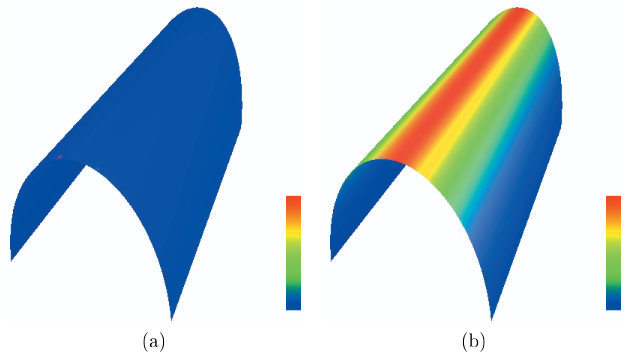
\includegraphics[width=0.9\textwidth]{../resources/curvature/gaussian_mean_k.png}
	\caption{This Comparison of Gaussian (a) and mean (b) curvature demonstrates how a surface that bends in only one direction will have 0 Gaussian curvature, whereas the mean curvature will vary with that direction~\cite{Imp_k_estimation_for_WS}.}
	\label{fig:mean_gauss_k} % NOTE: Label should be declared after caption
\end{figure}

\subsection{Root Mean Square Curvature}
Pulla et al. compared different types of curvature for the purpose of Watershed segmentation and found that although the absolute curvature produced the best results, the root mean square curvature produced similar results and was less computationally expensive.
The root mean square curvature is as the name implies, the square root of the average of the principal curvatures squared:
\begin{equation}
	\kappa_{rms} = \sqrt{\frac{\kappa_1^2 + \kappa_2^2}{2}}.
\end{equation}
% They compared different measures of curvature for this purpose and found that it was approximately as good as absolute curvature:
% \begin{equation*}
% 	\kappa_{abs} = |\kappa_1| + |\kappa_2|,
% \end{equation*}
They found $\kappa_{rms}$ cheaper to compute than the absolute curvature because they computed it from the mean and Gaussian curvatures:
\begin{equation*}
	\kappa_{rms} = \sqrt{4H^2 - 2K},
\end{equation*}
where $H$ and $K$ are the same mean and Gaussian curvatures explained above.
% RMS curvature was used during developement prior to implementing the derivative of curvature.

\subsection{Derivative of Curvature}
Through testing it was proposed that supplying the derivative of curvature instead of the curvature itself to watershed segmentation would better preserve the boundaries between semantic regions.
Rusinkiewicz proposes a method of taking the derivative of the curvature tensor~\cite{SRTensor}.
Because watershed segmentation expects a single value rather than a tensor, the magnitude of the derivative of the curvature tensor was approximated as the sum of squares of said tensor.

\section{Surface Regression}
The second high level step within \textit{3D Segmentation} is \textit{Surface Classification}, which attempts to classify the mesh segments yielded by Watershed segmentation as belonging to one of the defined geometric primitives.
Fitting 3D points to the various primitives was a part of \textit{Surface Classification}, initially as a means of confirming an initial shape primitive estimation, and later as means of direct shape primitive classification.
In both uses the regression results were confirmed by comparing the error value, obtained from the difference between the fitted primitive and the set of 3D points, to a pre-defined threshold.
The methods to perform and validate regression on the shape primitives implemented in this work are described in the following sections.

\subsection{Planar Regression}\label{sec:planar_regression}
A plane may be defined by a normal vector and a point on the plane.
% To perform planar regression on a set of 3D points principal component analysis is used to
Given a set of 3D points, principal component analysis (PCA) can be used to calculate the plane's normal vector as the PCA's least principal component.
% Given a set of 3D points, the least principal component from a PCA of the points is the regression plane's normal vector.
% That it, the direction that explains the least variance of the 3D points ... is the most significant for the normal vec?
The mean of the points is sufficient to produce the intersection point on the plane.
Calculating the error of such a regression is done by computing the distance from each point to the plane and calculating the root mean square of said distances like so:
\begin{equation}
	e_{RMSE} = \left(\frac{1}{N}\sum_{i}^{N}d_i^2 \right)^{\frac{1}{2}}.
\end{equation}
% The distance from a point $p_i$ to a plane described by point $p_P$ and normalized normal vector $\vec{n}$ may be calculated by transforming the point $p_i$ to the plane's coordinate system, with the origin at $p_P$ and which $\vec{n} = \vec{e_z}$.
The distance from a point $p_i$ to a plane described by point $p_P$ and normalized normal vector $\vec{n}$ may be calculated by transforming the target point to the plane's coordinate system, and taking the transformed point's $z$ coordinate as the distance.
% The distance from a point $p_i$ to a plane may be calculated by transforming the target point to the plane's coordinate system, with the origin at $p_P$ and which $\vec{n} = \vec{e_z}$:
\begin{equation}
	\prescript{P}{}p_i = \prescript{P}{}T_0 \prescript{0}{}p_i
\end{equation}
\begin{equation}
	d_i = \vec{e_z} \cdot \prescript{P}{}p_i
\end{equation}
where $\prescript{P}{}T_0$ is the homogeneous transformation matrix from global to planar coordinate systems.
Alternatively, if there is no other reason to compute the transformation matrix for the plane's local coordinate system, it is simpler to calculate the point-plane distance as the dot product of the plane normal with the vector $p_i - p_P$ as shown:
\begin{equation}
	d_i = \langle p_i - p_P, \vec{n}\rangle,
\end{equation}

\subsection{Cylindric Regression}
Cylinders in this context can be understood as an extruded conic section.
While there are methods of ascertaining (? better word?) a cylinder from a mere collection of 3D points~\cite{PCL_cyl_regression}, the process employed here was simplified by exploiting the mesh's normals.
For a cylindric mesh of constant radius with vertex normals, the normals will all be perpendicular to the main axis.
Thus, the least principal component from a PCA performed on the mesh's normals will yield a vector along the main axis.
From here a coordinate system may be created such that the z axis is the cylinder's main axis.
The origin of the cylindric coordinate system is for cylindric, and thus conic regression, inconsequential, but is typically set initially to the mean point position of the mesh.
Next, the mesh vertices are projected onto the XY plane of the cylinder's coordinate system, so that the specific type of conic may be deduced.
The general equation of a conic is:
\begin{equation}\label{eq:gen_conic}
	Ax^2 + Bxy + Cy^2 + Dx + Ey + F = 0.
\end{equation}
% Treating this as the error function to be minimized via least squares
Fitting a given set of 3D points to this equation can be achieved via total least squares.
Rosin shows that it is useful to set $F=1$~\cite{Ellipse_least_squares}, both to normalize the equation, and to avoid the trivial solution
\begin{equation}
	A = B = C = D = E = F = 0.
\end{equation}
Once the coefficients have been obtained, the specific type of conic represented by the points may be discerned by the determinant
\begin{equation*}
	B^2 - 4AC.
\end{equation*}
The specific method and equations to check the validity of the conic regression depend on the type of conic.

\subsubsection{Elliptic Regression}\label{sec:elliptic_reg}
For $B^2 - 4AC < 0$ the set of points represent an ellipse.
Computing the distance from a given point to an ellipse or other conic shape is non-trivial and, at the time of writing, no exact algebraic solution was found.
In place of an exact distance function, the sum of squared residuals was used throughout most of the project's timeline.
For example, a point on a conic section should satisfy Equation \ref{eq:gen_conic}, but for a point \textit{almost} on a conic section, the result will be non-zero:
\begin{equation}
	R(x,y) = Ax^2 + Bxy + Cy^2 + Dx + Ey + F \neq 0,
\end{equation}
where $R(x,y)$ is known as the residual. The error function then becomes
\begin{equation}
	e = \sum_i \left(Ax_i^2 + Bx_i y_i + Cy_i^2 + Dx_i + Ey_i + F\right)^2.
\end{equation}
While easy to calculate, this value is unreliable as an indicator of whether or not the given surface is actually a conic surface.
During testing cases were encountered in which obviously non-cylindric surfaces yielded extremely low error values, resulting in false positives.
This realization fueled the need for a proper point-to-ellipse distance function.

Eberly~\cite{GeoTools_pt_to_ellipse} shows that for an origin-centered axis-aligned ellipse described by major and minor diameters $a$ and $b$, and a target point $(x_p, y_p)$, the distance $t$ from the target point to the ellipse must satisfy the equation
\begin{equation}\label{eq:ellipse_dist}
	F(t) = \left(\frac{a x_p}{t + a^2}\right)^2 + \left(\frac{b y_p}{t + b^2}\right)^2 - 1 = 0.
\end{equation}
Eberly also compares 3 methods of solving Equation \ref{eq:ellipse_dist} for $t$, concluding that the bisection method is the most robust.

\subsubsection{Parabolic and Hyperbolic Regression}
% TODO: return to this, improve it.?
The functionality to perform parabolic or hyperbolic regression was omitted from this work due to time constraints.

(? I could layout how to compute the distance and thus error for at least a parabola, but is it worth it if it is not implemented? it is safe to assume the vast majority of curves encountered will be circular, and if not circular then elliptic...)

\section{UV Mapping}
\begin{figure}[htb]
	\centering
	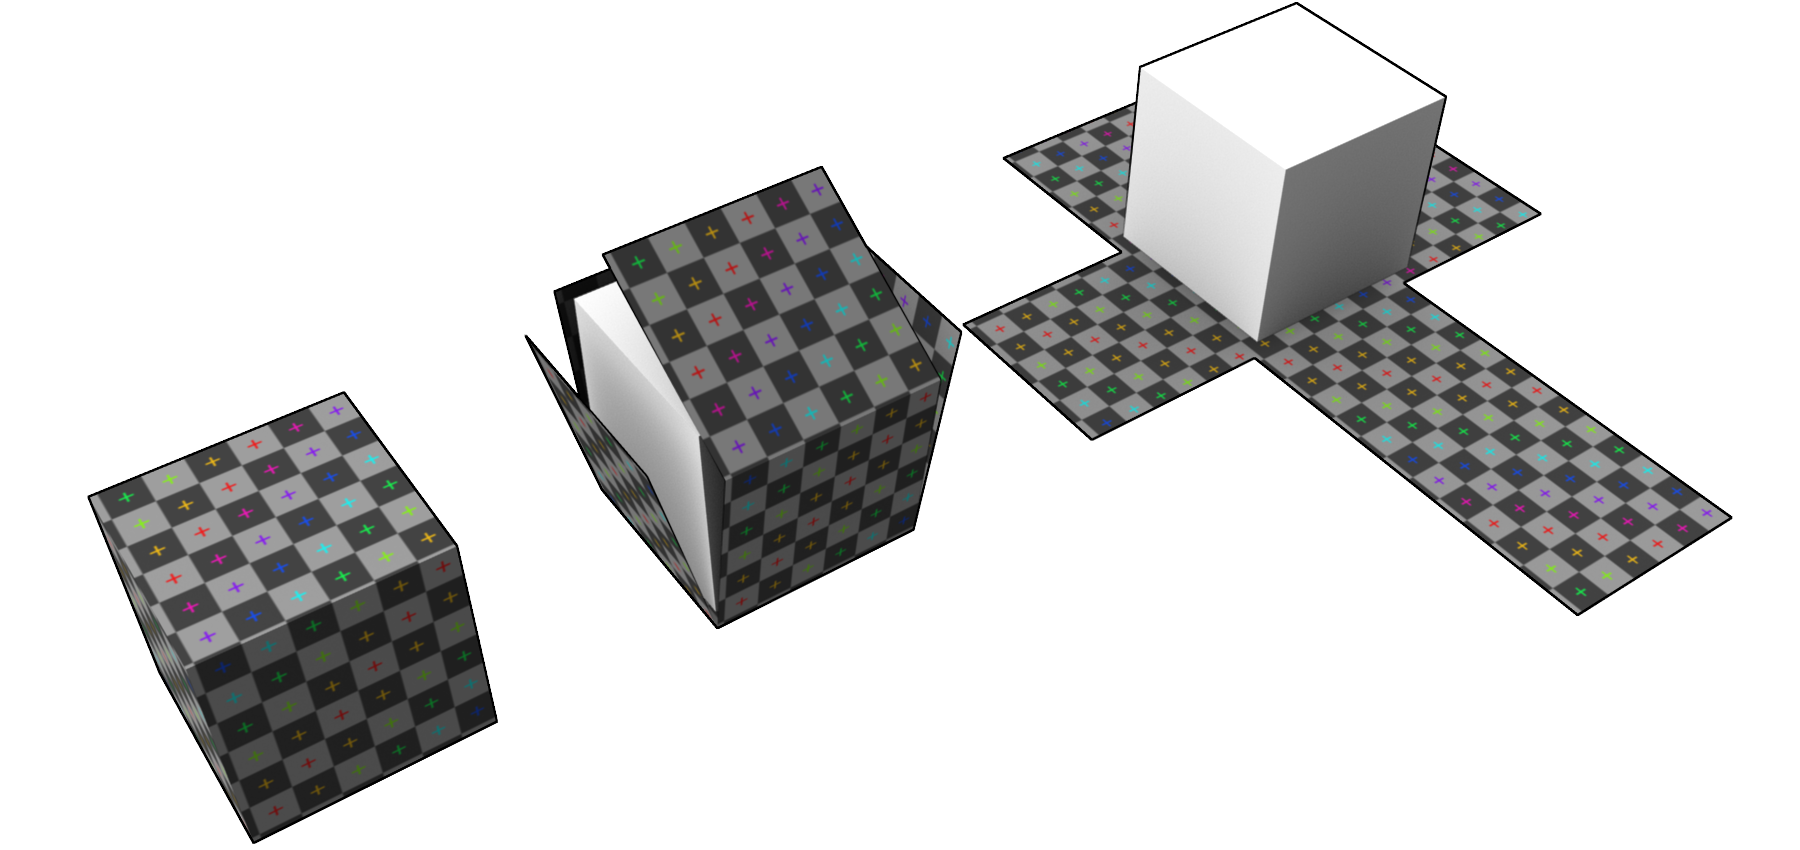
\includegraphics[width=0.65\textwidth]{../resources/cube_UV_unwrapping.png}
	\caption{Visual depiction of a cube's UV map being unwrapped~\cite{UV_map_cube_img}. }
	\label{fig:uv_map_cube}
	% NOTE: image requested by HK
\end{figure}
UV Mapping is the process of projecting a surface from 3D to 2D, effectively ``unwrapping'' the 3D surface.
UV maps are used extensively in 3D modeling and computer graphics.
Figure \ref{fig:uv_map_cube} shows the UV map of a cube being unwrapped.
Within the context of this work the primary purpose of UV maps are to handle the transformation of points from global to surface coordinates.
The plan was to have a UV map for each shape primitive to use during the \textit{Geometry Simplification} and \textit{Cellular Path Planning} high level steps.
% The functions a "UV-Map" in the code accomplishes:
	% Eigen::Vector2d xyz_to_uv(const Eigen::Vector3d& vec3) const;
	% Eigen::Vector3d uv_to_xyz(const Eigen::Vector2d& vec2) const;
	% Eigen::Vector3d pt_dir_intersection(
	% 	const Eigen::Vector3d& pt, const Eigen::Vector3d& dir) const;
	% Eigen::Vector3d surface_normal_at_pt(const Eigen::Vector3d& pt) const;
	% Eigen::Vector3d theta_to_RxRyRz(double theta) const;

The UV map for planar surfaces is trivial, as the 3D surface is already ``unwrapped''.
% TODO: ask about this
% (? if necessary i can explain in greater detail, but it seems superfluous...)

\subsection{Cylindric Surfaces}
For the purposes of this project, cylindric surfaces is restricted to extruded ellipses.
The process is first described for a circular cylinder, and then expanded to a generic ellipse.

\subsubsection{Circular Cylinders}
The transformation matrix $\prescript{c}{}T_0$ is the core of a circular cylindric UV map.
The z axis of $\prescript{c}{}T_0$ aligns with the cylinder's axis, and its origin is positioned at one end of the cylinder.
This can be observed in Figure \ref{sfig:gl_ccyl_transformation} below.
The transformation procedure is described visually in Figure \ref{fig:gl_ccyl_transform_steps}, and textually below.
\begin{figure}[htb]
	\centering
	\begin{subfigure}[b]{0.3\textwidth}
		\centering
\begin{tikzpicture}[scale=1.0]
	% CSYS
	\draw[->] (0,0) -- +(210:1.5) node[left] {X};
	\draw[->] (0,0) -- +(-30:1.5) node[right] {Y};
	\draw[->] (0,0) -- (0,1.5) node[above] {Z};
	% Cylinder
	\node[cylinder,shape border rotate=90,
		aspect=2.5, minimum height=20mm, minimum width=20mm,
		draw=blue!60] at (0,0.0) {};
	% Point
	\fill[purple] (1,0.5) circle[radius=3pt];
\end{tikzpicture}
		\caption{%
Step 1: Transform point to cylinder coordinates.
\begin{equation*}
	\prescript{c}{}p = \prescript{c}{}T_0 \prescript{0}{}p
\end{equation*}
}
		\label{sfig:gl_ccyl_transformation}
	\end{subfigure}
	\hfill
	\begin{subfigure}[b]{0.3\textwidth}
		\centering
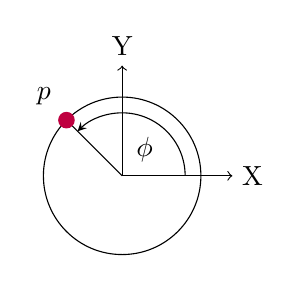
\begin{tikzpicture}[scale=1.0]
	% CSYS
	\draw[thin,->] (0,0) -- (1.4,0) node[right] {X};
	\draw[thin,->] (0,0) -- (0,1.4) node[above] {Y};
	% Cylinder -> Circle
	\draw (0,0) circle[radius=10mm,blue];
	% Point
	\node[circle,minimum size=6pt,fill=purple,inner sep=0, outer sep=0,label=135:$p$] (p1) at (135:10mm) {};
	% arrow and angle
	\draw (0,0) -- (p1);
	\draw[-stealth,black] (8mm,0) arc[start angle=0, end angle=135, radius=8mm]
		node[pos=0.37,below left] {$\phi$};
\end{tikzpicture}
		\caption{%
Step 2: Calculate $\phi$ using the point's x and y.
\begin{equation*}
	\phi = \arctan \frac{y}{x}
\end{equation*}
}
		% \label{fig:tangent_on_curve}
	\end{subfigure}
	\hfill
	\begin{subfigure}[b]{0.3\textwidth}
		\centering
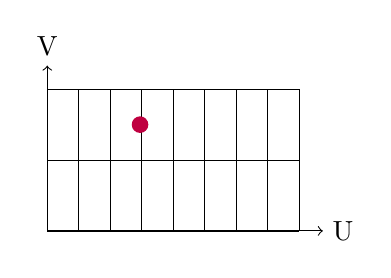
\begin{tikzpicture}[scale=1.0]
	% CSYS
	\draw[thin,->] (0,0) -- (3.5,0) node[right] {U};
	\draw[thin,->] (0,0) -- (0,2.1) node[above] {V};
	% Grid to represent unwrapped surface
	\draw[xstep=4mm,ystep=9mm,very thin] (0,0) grid (3.2,1.8);
	% Point
	\fill[purple] (1.178,1.35) circle[radius=3pt];
\end{tikzpicture}
		\caption{%
Step 3: Calculate UV coordinates.
% Point $\prescript{c}{}p$ shown on the unwrapped cylinder.
\begin{equation*}
	p(u,v) = (L \frac{\phi}{2\pi}, \prescript{c}{}p\text{.z})
\end{equation*}
}
		% \label{fig:tangent_on_curve}
	\end{subfigure}
	\caption{Graphic depiction of a point transformed from global to cylinder surface coordinates.}
	\label{fig:gl_ccyl_transform_steps}
\end{figure}

First the point is transformed to the cylinder's coordinate system in $R^3$.
From here the $x$ and $y$ coordinates of the point are used to calculate the angle $\phi$ measured from the $x$ axis.
The point's $u$ coordinate is calculated as the ratio of $\phi$ to its perimeter using
\begin{equation}\label{eq:cyl_u_coord}
	u = L \frac{\phi}{2\pi},
\end{equation}
where $L$ is the cylinder's perimeter: $2\pi r$.
% $\phi$ is used to calculate the arc length position of $\prescript{c}{}p$ along the cylinder's perimeter, which becomes its $u$ position in surface coordinates.
The point's $z$ in the cylinder's coordinate system becomes its $v$ coordinate in surface coordinates.

To transform a point in surface coordinates to $R^3$, the steps above must be reversed.
Solving Equation \ref{eq:cyl_u_coord} for $\phi$, the point's $u$ coordinate is converted back to the angle $\phi$:
\begin{equation*}
	\phi = 2\pi \frac{u}{L}.
\end{equation*}
Next the point's position in cylinder coordinates are calculated as
\begin{equation*}
	\prescript{c}{}p(x,y,z) = (r \cos \phi, r \sin \phi, v)
\end{equation*}
where $r$ is the circle's radius.
Finally, the point may be transformed from the cylindric to the global frame of reference using the transformation matrix $\prescript{0}{}T_c$.

\subsubsection{Elliptic Cylinders}
An ellipse is merely a circle that has been stretched.
Because of this, the procedure to transform a point from $R^3$ to the surface coordinates of an elliptic cylinder is the same as that of the circular cylinder, save for some different equations.
Here, the elliptic UV map contains transformation matrix $\prescript{e}{}T_0$, with its z axis aligned with the cylinder's main axis, x axis aligned with the ellipse's major axis, and origin centered on the ellipse.
Recall that the general equation of an ellipse is
\begin{equation*}
	\frac{x^2}{a^2} + \frac{y^2}{b^2} = 1,
\end{equation*}
where $a$ is the radius along the major axis, and $b$ is the radius along the minor axis.
The transformation procedure is described visually in Figure \ref{fig:gl_ecyl_transform_steps}, and textually further below.

\begin{figure}[htb]
	\centering
	\begin{subfigure}[b]{0.3\textwidth}
		\centering
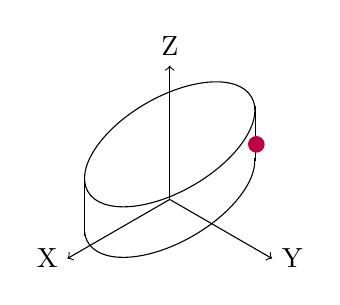
\begin{tikzpicture}[scale=1.0]
	% \draw[step=10mm,gray!50,very thin] (-2.2,-0.2) grid (2.2,3.2);
	% CSYS
	\draw[->] (0,0) -- +(210:1.5) node[left] {X};
	\draw[->] (0,0) -- +(-30:1.5) node[right] {Y};
	\draw[->] (0,0) -- (0,1.7) node[above] {Z};
	% Ellipse(s)
	% \draw[gray!50] (0,0.0) ellipse[x radius=12mm, y radius=6mm,rotate=30];
	\draw[] (24:11.9mm) -- +(0,0.7);
	\draw[] (203:11.8mm) -- +(0,0.7);
	\draw (26:12.0mm) {[rotate=30] arc
		[start angle=-13, delta angle=-180, x radius=12mm, y radius=6mm,rotate=30]};
	\draw[] (0,0.7) ellipse[x radius=12mm, y radius=6mm,rotate=30];
	% Point
	\fill[purple] (1.1,0.7) circle[radius=3pt];
\end{tikzpicture}
		\caption{%
Step 1: Transform point to cylinder coordinates.
\begin{equation*}
	\prescript{e}{}p = \prescript{e}{}T_0 \prescript{0}{}p
\end{equation*}
}
		% \label{sfig:gl_ecyl_transformation}
	\end{subfigure}
	\hfill
	\begin{subfigure}[b]{0.3\textwidth}
		\centering
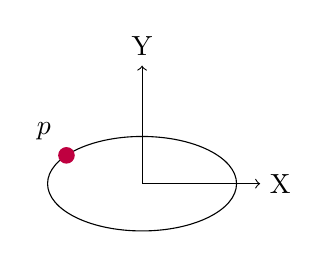
\begin{tikzpicture}[scale=1.0]
	% \draw[step=10mm,gray!50,very thin] (-2.2,-0.2) grid (2.2,3.2);
	% CSYS
	\draw[thin,->] (0,0) -- (1.5,0) node[right] {X};
	\draw[thin,->] (0,0) -- (0,1.5) node[above] {Y};
	% Cylinder -> Circle
	\draw[] (0,0) ellipse[x radius=12mm, y radius=6mm];
	% Point
	\node[circle,minimum size=6pt,fill=purple,inner sep=0, outer sep=0,label=135:$p$] at (-0.96,0.36) {};
	% arrow and angle
	% \draw (0,0) -- (p1);
	% \draw (8mm,0) arc [->,start angle=0, end angle=135, radius=8mm];
\end{tikzpicture}
		\caption{%
Step 2: Calculate $\phi$ using the point's x and y.
\begin{equation*}
	\phi = \arctan \frac{y/b}{x/a}
\end{equation*}
}
		\label{sfig:ellipse_xy_coords}
	\end{subfigure}
	\hfill
	\begin{subfigure}[b]{0.3\textwidth}
		\centering
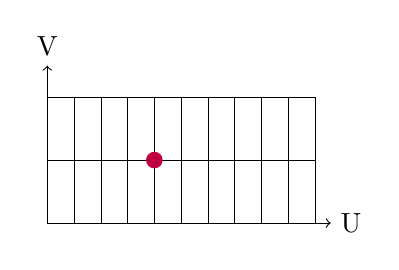
\begin{tikzpicture}[scale=1.0]
	% CSYS
	\draw[thin,->] (0,0) -- (3.6,0) node[right] {U};
	\draw[thin,->] (0,0) -- (0,2.0) node[above] {V};
	% Grid to represent unwrapped surface
	\draw[xstep=3.4mm,ystep=8mm,very thin] (0,0) grid (3.4,1.6);
	% Point
	\fill[purple] (1.36,0.8) circle[radius=3pt];
\end{tikzpicture}
		\caption{%
Step 3: Calculate UV coordinates.
% Point $\prescript{c}{}p$ shown on the unwrapped cylinder.
\begin{equation*}
	p(u,v) = (L \frac{\phi}{2\pi}, \prescript{e}{}p\text{.z})
\end{equation*}
}
		% \label{fig:tangent_on_curve}
	\end{subfigure}
	\caption{Graphic depiction of a point transformed from global to cylinder surface coordinates.}
	\label{fig:gl_ecyl_transform_steps}
\end{figure}

The first step remains unchanged: Transform the point to the cylinder's coordinate system.
The objective of the second step remains calculating the arc angle $\phi$, but here the coordinates must be scaled by their corresponding radii to account for the ellipse's eccentricity.
Note that for an ellipse $\phi$ is not equivalent to the angle to the point measured from the local $x$ axis, as that would be $\arctan y/x$.
Hence why there is no line or marker indicating $\phi$ in Figure \ref{sfig:ellipse_xy_coords}.

Performing the reverse transformation is equivalent to that of the circular cylinder, with the exception that the individual radii must be used instead of the singular radius $r$:
\begin{equation*}
	\prescript{c}{}p(x,y,z) = (a \cos \phi, b \sin \phi, v).
\end{equation*}
From here, the point is transformed from cylindric to global coordinates using $\prescript{}{}T_e$.

\iffalse
To obtain a vector perpendicular to a point on the ellipse, the derivative of said point is rotated 90 degrees.
The point, as a function of the angle $\theta$:
\begin{equation}
	(x,y) = (a\cos\theta, b\sin\theta)
\end{equation}
The derivative thereof:
\begin{equation}
	\frac{d}{d\theta}(x,y) = (-a\sin\theta, b\cos\theta)
\end{equation}
Rotated -90 degrees:
\begin{equation}
	\text{Rot}_{90}\frac{d}{d\theta}(x,y) = (b\cos\theta, a\sin\theta)
\end{equation}

\subsubsection{Parabolic and Hyperbolic Surfaces}
Parabolas are much simpler than and ellipses and hyperbolas, as can be seen by the following equations.
The parametric general equation of a parabola is:
\begin{equation}
	-\sin\theta x + \cos\theta y = \frac{1}{4f}(\cos\theta x + \sin\theta y - h)^2 + k
\end{equation}
To solve for the conic parameters of a parabola the general equation's quadratic term is expanded and like terms gathered:
\begin{multline*}
	-\sin\theta x + \cos\theta y = \frac{1}{4f}(\cos^2\theta x^2 + \cos\theta\sin\theta xy \\
	- h \cos\theta x + \cos\theta\sin\theta xy + \sin^2\theta y^2 - h\sin\theta y - h \cos\theta x - h \sin\theta y + h^2) + k
\end{multline*}
\begin{multline*}
	\frac{\cos^2\theta}{4f} x^2 + \frac{2\cos\theta\sin\theta}{4f} xy + \frac{\sin^2\theta}{4f} y^2 \\
	+ \left(\sin\theta - \frac{2h \cos\theta}{4f}\right)x + \left(\cos\theta - \frac{2h \sin\theta}{4f}\right)y + \frac{h^2}{4f} + k = 0
\end{multline*}
\begin{align}
	A &= \frac{\cos^2\theta}{4f} \\
	B &= \frac{2\cos\theta\sin\theta}{4f} \\
	C &= \frac{\sin^2\theta}{4f} \\
	D &= \sin\theta - \frac{2h \cos\theta}{4f} \\
	E &= \cos\theta - \frac{2h \sin\theta}{4f} \\
	F &= \frac{h^2}{4f} + k
\end{align}

\subsubsection{Hyperbolic Surface}
\begin{equation}
\begin{split}
	\frac{(\cos\theta(x-h) + \sin\theta(y-k))^2}{a^2} - \frac{(\cos\theta(y-k) + \sin\theta(x-h))^2}{b^2} &= 1 \\
	\frac{(x_c + y_s)^2}{a^2} - \frac{(y_c + x_s)^2}{b^2} &= 1 \\
	b^2(x_c^2 + 2x_c y_s + y_s^2) - a^2(y_c^2 + 2 x_s y_c + x_s^2) &= a^2 b^2 \\
	b^2 x_c^2 + 2 b^2 x_c y_s + b^2 y_s^2 - a^2 y_c^2 - 2 a^2 x_s y_c - a^2 x_s^2 - a^2 b^2 &= 0 \\
	b^2 x_c^2 - a^2 x_s^2 + 2 b^2 x_c y_s - 2 a^2 x_s y_c + b^2 y_s^2 - a^2 y_c^2 - a^2 b^2 &= 0 \\
\end{split}
\end{equation}
\begin{multline*}
	b^2 (\cos\theta(x-h))^2 - a^2 (\sin\theta(x-h))^2 \\
	+ 2 b^2 \cos\theta(x-h) \sin\theta(y-k) - 2 a^2 \sin\theta(x-h) \cos\theta(y-k) \\
	+ b^2 (\sin\theta(y-k))^2 - a^2 (\cos\theta(y-k))^2 - a^2 b^2 = 0
\end{multline*}
\begin{multline*}
	(b^2 \cos^2\theta - a^2 \sin^2\theta)(x-h)^2 \\
	+ 2 \cos\theta\sin\theta(b^2 - a^2)(x-h)(y-k) \\
	+ (b^2 \sin^2\theta - a^2 \cos^2\theta)(y-k)^2 - a^2 b^2 = 0
\end{multline*}
\begin{equation*}
	\begin{split}
		c_1(x-h)^2 + c_2(x-h)(y-k) + c_3(y-k)^2 - a^2 b^2 &= 0 \\
		c_1(x^2-2hx + h^2) + c_2(xy-hy-kx+hk) + c_3(y^2-2ky+k^2) - a^2 b^2 &= 0 \\
		c_1 x^2 + c_2 xy + c_3 y^2 + (-2h c_1 -k c_2) x + (-h c_2 -2k c_3)y + c_1 h^2 + c_2 hk + c_3 k^2 - a^2 b^2 &= 0 \\
	\end{split}
\end{equation*}
\begin{align*}
	A &= c_1 = b^2 \cos^2\theta - a^2 \sin^2\theta \\
	B &= c_2 = 2 \cos\theta\sin\theta(b^2 - a^2) \\
	C &= c_3 = b^2 \sin^2\theta - a^2 \cos^2\theta \\
	D &= (-2h c_1 -k c_2) \\
	E &= (-h c_2 -2k c_3) \\
	F &= c_1 h^2 + c_2 hk + c_3 k^2 - a^2 b^2
\end{align*}
Now to solve for $a$, $b$, and $\theta$:
Solving $A$ for $b^2$:
\begin{equation}
	\begin{split}
		A &= b^2 \cos^2\theta - a^2 \sin^2\theta \\
		b^2 &= \frac{A}{\cos^2\theta} + a^2\tan^2\theta \\
	\end{split}
\end{equation}
Setting 3.6 into $C$ and solving for $a^2$:
\begin{equation}
	\begin{split}
		C &= b^2 \sin^2\theta - a^2 \cos^2\theta \\
		a^2 &= -\frac{C}{\cos^2\theta} + b^2\tan^2\theta \\
		a^2 &= -\frac{C}{\cos^2\theta} + \left(\frac{A}{\cos^2\theta} + a^2\tan^2\theta\right)\tan^2\theta \\
		\cos^4\theta a^2 &= -C\cos^2\theta + A\cos^2\theta + \sin^4\theta a^2 \\
		(\cos^4\theta - \sin^4\theta) a^2  &= \cos^2\theta(A-C) \\
		a^2  &= \frac{\cos^2\theta(A-C)}{(\cos^4\theta - \sin^4\theta)} \\
	\end{split}
\end{equation}
Setting 3.6 into $B$:
\begin{equation}
	\begin{split}
		B &= 2 \cos\theta\sin\theta(\frac{A}{\cos^2\theta} + a^2\tan^2\theta - a^2) \\
		\cos^2\theta B &= 2 \cos\theta\sin\theta(A + (\sin^2\theta - \cos^2\theta) a^2) \\
	\end{split}
\end{equation}
Setting 3.7 into 3.8:
\begin{equation}
	\begin{split}
		\cos^2\theta B &= 2 \cos\theta\sin\theta(A + (\sin^2\theta - \cos^2\theta) \frac{\cos^2\theta(A-C)}{(\cos^4\theta - \sin^4\theta)}) \\
	\end{split}
\end{equation}
\fi

\section{Ramer-Douglas-Peucker Algorithm}
The Ramer-Douglas-Peucker (RDP) algorithm is a method to interatively simplify a line defined by a set of points~\cite{RDP_line_reduction_DP, RDP_line_reduction_R}.
The only arguments to RDP are a list of points and a tolerance width, within which points will be considered unnecessary and discarded.
% The algorithm looks at a list of points, draws an imaginary line from the first to the last, finds the point with the farthest normal distance to the comparison line, and if the point's distance to the comparison line is greater than a pre-defined tolerance width, splits the lin
The algorithm iteratively finds the point farthest from the straight line from point 0 to n-1, and if said distance is greater than the tolerance width, the line is split at the farthest point and the line sections before and after the split are reconsidered individually.
The procedure is described in greater detail in Algorithm~\ref{alg:RDP}.

\begin{algorithm}[htb]
\caption{Ramer-Douglas-Peucker}\label{alg:RDP}
\begin{algorithmic}[1]
\Function{SimplifyLineRDP}{points $P$, real $w$}
	\State new list $P_{core}$\Comment{To store the important point indices}
	\State new RDPNode $n_0 \leftarrow$ RDPNode($P$.first, $P$.last)
	\State new list $N_{stack} \leftarrow n_0$
	\While{$N_{stack}$ not empty}
		\State new RDPNode $n \leftarrow N_{stack}$.last
		\State $N_{stack}$.popLast()
		\State new uint $i \leftarrow$ index of point farthest from $n$.line
		\State new real $d \leftarrow$ distance of $P$[$i$] from $n$.line
		\If{$d \le w$} \Comment{If farthest point is within tolerance}
			\State $P_{core}$.append($n$.srcPt) \Comment{line section is complete}
			\State \textbf{continue}
		\EndIf
		\State new RDPNode $n_{left} \leftarrow$ RDPNode($n$.srcPt, $P$[$i$])
		\State new RDPNode $n_{right} \leftarrow$ RDPNode($P$[$i$], $n$.endPt)
		\State $N_{stack}$.append($n_{right}$)
		\State $N_{stack}$.append($n_{left}$)
	\EndWhile
	\State $P_{core}$.append($P$.last)
	\State \textbf{return} $P_{core}$
\EndFunction
\end{algorithmic}
\end{algorithm}

The RDP implementation used in this work uses a struct \textbf{RDPNode} that represents a section of the line.
It contains a start and end point, as well as a line spanning these two points.
A stack is used to manage the \textbf{RDPNode}s.
In each iteration of the \verb|while| loop, starting on line 5, the item at the top of the stack is removed and stored in $n$.
The point farthest from this line section is found, and on line 10 the distance thereof is compared against the tolerance width.
If the perpendicular distance is within the tolerance width then the current line section is complete and the initial point in the section is added to $P_{core}$ (line 11).
If not, then the current line section is split at the farthest point, with the two new sections represented by RDPNodes $n_{left}$ and $n_{right}$.
These are then placed on the stack, $n_{right}$ first, so that $n_{left}$ is processed next, ensuring the list of important points $P_{core}$ is always sorted.
After the \textbf{RDPNode} stack is exhausted the last point in $P$ is appended to $P_{core}$ because only the start point in each node is added to $P_{core}$.
An alternative implementation that uses recursion may be found on wikipedia.

\section{Traveling Salesman Problem}
The Traveling Salesman Problem (TSP) is a well known problem in combinatorial optimization.
The original problem was posed as the following:
A salesman wishes to visit every city in a given region once, to spend the least amount of time traveling between cities, and to end at his home city.
It was initially formulated in the 1800s by mathematicians William Rowan Hamilton and Thomas Kirkman~\cite{Graph_theory}.
The problem can be stripped down to simply the optimal round-trip traversal of a set of nodes in a graph, where the traversal represents the salesman's movement, and each node represents a city.
It can be shown~\cite{TSP_in_pursuit_of} that for $n$ nodes the number of possible route permutations is
\begin{equation*}
	n_{\text{routes}} = (n-1)!.
\end{equation*}
For the vast majority of applications symmetric node-to-node costs can be assumed, and the number of permutations is reduced to \textit{only}
\begin{equation*}
	n_{\text{routes}} = \frac{(n-1)!}{2}.
\end{equation*}
The number of real world TSP applications is similarly large~\cite{TSP_theory_applications}, ranging from determining the drill order of holes in printed circuit board manufacturing~\cite{TSP_PCB_manufacturing}, to mail delivery and vehicle routing in general~\cite{TSP_mail_delivery}, to X-ray crystallography~\cite{TSP_xray_crystallography}.
The algorithm described in this work produces a set of convex surfaces from the target object.
Within each convex surface region a simple path is planned.
% NOTE the verb tense/case! "would" because it is not implemented
It is the traversal of these surface regions that would be formulated as a TSP with the distance between each region and the change in end-effector orientation serving as the travel costs.
Considering only the traversal of the surface regions, the start and end nodes need not be the same, and the situation can be modeled as a modified TSP.
The common way to modify a TSP to achieve different start and end nodes is to introduce a dummy node with 0-cost edges to the other nodes~\cite{TSP_dummy_node_mod}.
After insertion of the dummy node, the TSP can be solved like normal.
Once the TSP has been solved the nodes adjacent to the dummy node are the start and end nodes.
If the robot's starting or home position is included as a node, the application can be handled as a classic TSP.

